The underlying mechanism which causes timing noise is not understood. Since the
first discussions in \citet{Boynton1972} multiple models have been proposed
which are able to describe some of the features. However, the variety of ways
timing noise manifests and the uncertainty in the mechanisms at work have made
it difficult for any conclusive statements to be made about the models. A
complete understanding of timing noise must not only explain the observed
variations, but also remain consistent with our understanding of neutron stars
derived from other observations such as glitches. A complicating factor in
understanding timing noise is that the observed features have timescales
similar to the duration that we have been able to observe pulsars; it is
therefore possible that observations which look like a random walk over a short
timescale, may in fact be periodic or something else entirely over longer
timescales.  Observations of new features prompt new models for timing noise;
as a result the timing noise interpretations have evolved with the
observations. In this section we will present an overview of these concepts and
the existing evidence which supports them.

\subsection{Random walk models}
\label{sec: TN interpretations random walk models}

Timing noise was first quantified and interpreted by \citet{Boynton1972} as a
Poisson like random walk in one of the phase, frequency, or spin-down. The
pulsar spins down according to the power law spin-down of equation \eqref{eqn:
power law spin-down} except that at random times the pulse phase, frequency, or
spin-down will undergo a sudden discontinuity. The waiting times between such events
are Poisson distributed with a rate $R$ such that over a period $T$ the number of
events follows a Poisson distribution with mean $RT$. All the jumps are
independent and the magnitudes are randomly distributed with means given by
$\langle\dP\rangle$, $\langle\dF\rangle$, and $\langle\dS\rangle$ for the phase,
frequency, and spin-down.

\citet{Boynton1972} and others since investigate the statistical properties of
such random walks by splitting the phase evolution into contributions from the
secular spin-down $\phi_{\mathrm{S}}$, as given by equation \eqref{eqn: Taylor
compact}, and contributions from the random walks $\Delta\phi_\mathrm{R}$. Such
that the total phase evolution is given by
\begin{equation}
    \phi = \phi_{\mathrm{S}} + \Delta\phi_{\mathrm{R}}.
\end{equation}
The three random walks can be written as the sum of $N$ individual events
occurring at times $t_{i}$
\begin{align}
    \Delta\phi_{\mathrm{R}} & = \s{i=1}{N}\Delta\phi_{i} H(t - t_{i})
     && \mathrm{(phase),} \\
    \Delta\phi_{\mathrm{R}} & = \s{i=1}{N}\Delta\f_{i} (t-t_{i})H(t - t_{i})
     && \mathrm{(frequency),} \\
    \Delta\phi_{\mathrm{R}} & = \s{i=1}{N}\frac{1}{2}\Delta\fdot_{i} (t-t_{i})^{2}H(t - t_{i})
     && \mathrm{(spin-down),}
\end{align}
where $H(t)$ is unit step function at $t=0$. It should be noted that here we are
treating the three types of noise separately such that timing noise residuals
from either a random walk in phase, frequency, or spin-down; work by \citet{Cordes1980}
extended this model to handle mixing between the types of noise.

Timing noise is the remainder having
fitted and subtracted a second order Taylor expansion. Provided the perturbations
of $\phi_{\mathrm{s}}$ are small then the remainder will be exactly given by
$\phi_{\mathrm{s}}$. Then, as described by \citet{Boynton1972} we can then
average over: the $\dP_{i}, \dF_{i}$ or $\dS_{i}$
distributions, the $t_{i}$ distribution, and the $N$ distributions to give
\begin{align}
    \langle \Delta\phi_{R} \rangle & = \langle \dP \rangle R T
    = S_{\mathrm{PN}}T && \mathrm{(phase),} \\
    \langle \Delta\phi_{R} \rangle & = \frac{1}{2}\langle \dF \rangle R T^{2}
    = \frac{1}{2}S_{\mathrm{FN}}T^{2} && \mathrm{(frequency),} \\
    \langle \Delta\phi_{R} \rangle & = \frac{1}{6}\langle \dS \rangle R T^{3}
    = \frac{1}{6}S_{\mathrm{SN}}T^{3} && \mathrm{(spin-down).}
\end{align}
Here we have implicitly defined the strength parameters which combine the rate
and averaged magnitude of jumps into a single quantity. Measurements of timing
noise, if they are discreet events, will observe the accumulation of many
individual events. As a result only the strength can be
measured, not the rate and average magnitude.

The three types of noise are distinguishable by their dependence on the
observation time $T$. The type of noise can be measured by translating this
into the dispersion measure of $\Delta\fddot$ after fitting a cubic, or by
inspection of the power spectrum.  \citet{Boynton1972} was able to categorise
the Crab pulsar as `frequency-like' noise.  They found that over a $5$~year
period the noise process was stationary and consistent with the frequency noise
hypothesis. No deterministic process could account for the timing residuals
strengthening their conviction that some random process was taking place.
However, they suggested that over longer periods the random walk will be
non-stationary due to either mixing with other types of walks, or decay of the
strength parameter with time.

The interpretation of timing noise as a Poisson random walk is a purely
empirical statistical model. It is however backed up for a rich variety of
possible substantive physical models.  A key feature of any physical random
walk model is that it must be able to produce both increases and decreases in
the relevant parameter. For this reason it is felt unlikely that mechanism
responsible for a random walk timing noise model is the same as model proposed
to explain glitches. Moreover, since it is assumed that the number of events
is large so that we can take a statistical average, this does not test if the
process is indeed discreet, or if it is continuous.

The first physical model was proposed by \citet{Boynton1972}, the noise process
consisted of the accretion of small lumps of matter onto the NS from the
interstellar medium. Lumps of matter fall randomly onto the surface of the star
causing either a spin-up or spin-down through the transfer of angular momentum.
After this many models were proposed such as starquakes and the random pinning
and unpinning of vortex lines; these were reviewed by \citet{Cordes1981} and
evaluated against observational constraints. Of these only three mechanisms
where found to be consistent with observations: crust breaking by vortex pinning, a
response to heat pulses, and luminosity related torque fluctuations. Since this
review, new random walk mechanisms have been proposed such as: variations in
the magnetospheric gap size \citep{Cheng1987}; the interference by debris entering
the magnetosphere \citep{Cordes2008}; and the accumulation of multiple micro-glitches
\citep{Janssen2006}. It would be a useful exercise to review both the new and
old mechanisms against the current observational catalogue since new and improved
observations may better constrain some of these physical models.

The first measurement of individual events was made by \citet{Cordes1985} who
identified $\sim20$ events in both frequency and spin-down which could not be
explained by a glitch. In the same work, considering 24 pulsars over a period
of~$\sim13$~years, the authors concluded that: the timing noise seen in the
data could not be explained solely by an idealised random walk processes in the
phase, or its derivatives. They suggested that most of the activity is due to a
mixture of events in the phase, frequency and/or frequency derivative.

A recent observational review of timing noise was performed by
\citet{Hobbs2010} for 366 pulsars, the authors do not comment on whether these
observations constrain random walk models. Instead, they conclude that, when
observed on sufficiently long time scales, the residuals which may before have
looked like a random walk, contained quasi-periodic features. It is impossible
to argue that this is not the case for pulsars which only display random-walk
features over current observation periods, since the quasi-periodicity may only
As such, the method of measuring the type and strength of timing noise depends
on the length and epoch of observation. This suggests a pure random walk
hypothesis is not entirely consistent with observations.

\subsection{Free precession}
\label{sec: free precession}

A mechanism which could quite naturally produce strictly periodic variations in the
observable features of a pulsar is \emph{free precession}. This occurs in any
non-spherical body for which the angular momentum is not aligned with a principle
axis of the moment of inertia. Such a circumstance could arise given the
chaotic birth of NSs. However, we must be clear that the timing noise induced by
precession alone would be strictly deterministic; this is something which we do
not observe.
It is instructive however to consider the mechanics of precession since it will
be visited later on.

In the simplest case imagine an biaxial body,
rotating about an axis $\Omega$. with a moment of inertia given by
\begin{equation}
    I = \left[\begin{array}{ccc}
            I_{0} & 0 & 0 \\
            0 & I_{0} & 0 \\
            0 & 0 & I_{0}(1 + \epsilon)
            \end{array}\right],
\end{equation}
where $\epsilon \ll 1$ is the measure of oblateness or prolateness.  If the
body is free from torques, then in the rotating frame of the body, Euler's
equations of motion \citep{Landau1969} are given by
\begin{equation}
    I\dot{\bm{\Omega}} + \bm{\Omega} \times \left(I\bm{\Omega}\right)=0.
\end{equation}
This is a system of three coupled ODEs. Writing the components of the spin
vector as $\bm{\Omega} = [\Omega_{x}, \Omega_{y}, \Omega{z}]$, we have the
set of equations:
\begin{align}
\dot{\Omega}_x = -\Omega_y\Omega_z, &&
\dot{\Omega}_y = \Omega_x \Omega_z, &&
\dot{\Omega}_z = 0
\end{align}
We can find a solution by first setting $\Omega_{z}=\mathrm{const}$.
We are then left with a set of
two coupled ODEs, solving these with appropriate initial conditions
the solutions take the form
\begin{align}
\begin{split}
    \Omega_{x} & = \Omega_{0}\sin(a_0)\sin\left(\Omega_{0}\cos(a_0)\epsilon t\right), \\
    \Omega_{y} & = \Omega_{0}\sin(a_0)\cos\left(\Omega_{0}\cos(a_0)\epsilon t\right),\\
    \Omega_{z} & = \Omega_0 \cos(a_0),
\label{eqn: free precession}
\end{split}
\end{align}
where $a_0$ is the angle between the spin-vector and the body frame $z$ axis and
$\Omega_0$ is the magnitude of the spin-vector.

We observe that the spin axis of the body will trace out a cone about the $z$
principle axis of the moment of inertia with a period of
$\frac{1}{\Omega_{z}\epsilon}$.  The half-angle of the cone is set by the
initial conditions and will not evolve. This is the motion of free precession
and is illustrated in figure \ref{fig: precession}.
\begin{figure}[htb]
\centering
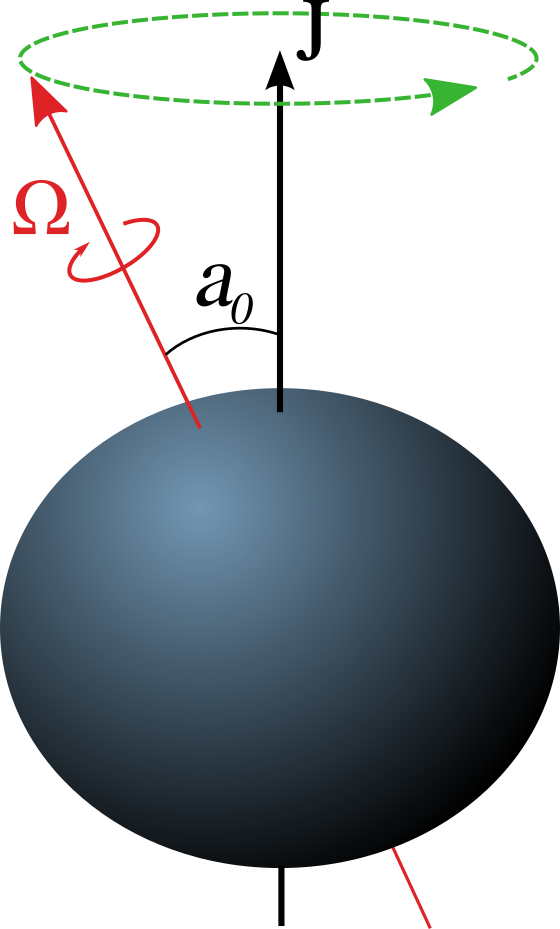
\includegraphics[scale=0.2]{Precession.png}
\caption{Illustration of free precession for a simple biaxial body. The spin
    axis $\spin$ traces out a cone about the angular momentum vector $\mathbf{J}$.}
\label{fig: precession}
\end{figure}•

Neutron stars are assumed to have a rigid crust, as such they may be
non-axially symmetric. Precession as a candidate to explain timing noise
fluctuations was first discussed by \citet{Ruderman1970}. He found that the
free precession period was, for reasonable values of the  ellipticity
$\epsilon$, able to explain periodic fluctuations in the Crab pulsar. Of the
known Neutron star physics, one of the few periodic mechanism that could
operate over the time-scales observed in timing residuals is free precession.

The superfluid unpinning interpretation for glitches poses a problem for
sustained free precession as an interpretation of timing noise. If correct then
the interior of a neutron star must contain a superfluid component pinned to
the crust.
It was shown by \citet{Shaham1977} that for perfect pinning the free precession
frequency and geometry were modified resulting in no slowly oscillating
long-lived modes. In the case of imperfect pinning \citet{Sedrakian1999} found
that long-lived modes existed, but were damped.

Despite the inconsistency with the superfluid pinning model for glitches,
evidence was presented by \citet{Stairs2000} of free precession in pulsar
B1828-11. They found the phase residuals and variations in the pulse profile
could be accounted for by precession. This was followed up by detailed
modelling of the effects by \citet{Akgun2006}.

Including the spin-down from an applied torque \citet{Cordes1993} noted that
free precession may be driven by fluctuations that counter the damping process;
in turn, the precession can drive torque fluctuations. The effect is most
noticeable in young pulsars.

Work by \citet{Jones2001} compared a model of free precession against the handful
of proposed observations of free precession. Their model included the feedback
between the torque and precession and required only the crust to undergo precession.
In all but one case such a model was found to be consistent with the observations.

In this work we will consider in detail the implications of precession for
neutron stars and develop some of the ideas discussed above.

\subsection{Two state switching}
\label{sec: two state switching}

Recently a new model has been proposed by \citet{Lyne2010} to explain the
observation that, over long time periods, the timing noise structure is
quasi-periodic. This began with the observation by \citet{Kramer2006} that the
pulses from PSR B1931+24 where intermittent: the pulsar acts as a normal pulsar
for $\sim10$~days and then switches off, being undetectable for $\sim25$~days,
before switching on again. Analysing the spin-down rate between the on and off
states, they determined the spin-down rate $\dot{\f}$ was $\sim50\%$ faster in
the on state. The figure illustrating this is reproduced in figure \ref{fig:
kramer 2006 fig2}.
\begin{figure}
    \centering
    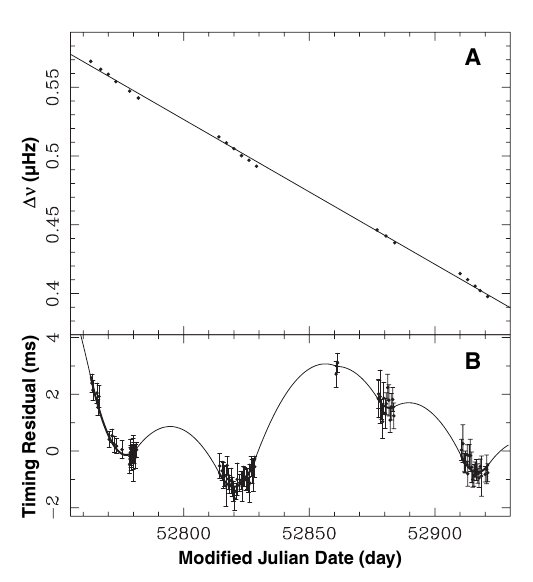
\includegraphics[width=.5\textwidth]{Kramer_2006_fig2}
    \caption{Figure taken from \citet{Kramer2006} showing the switched spin-down
             of pulsar PSR B1931+24}
    \label{fig: kramer 2006 fig2}
\end{figure}
In the  upper panel (\textbf{A}) the authors show the evolution of the
rotational frequency over a 160 day period encompassing several switching
events. The line shows the long-term spin-down of the pulsar while the dots show
individual measurements made during the on state. During these on states the
gradient of the reduction in frequency is increased, that is the spin-down has
increased. It is thought that measurements of the frequency in the off state
would produce a line with decreased spin-down connecting the dots. This is
accompanied by the timing residual measured over the same period in the lower
panel (\textbf{B}). This shows significant quasi-periodic modulations in sync
with the switching. This work proposed that the switching was a magnetospheric
phenomenon. The sharpness of the switches certainly requires something acting
on a short timescale and it intuitively makes sense that the greater spin-down
results from greater torque produced by the emissions observed during the on
state.

The authors of \citet{Lyne2010} then tested a range of other pulsars and
presented a study of 17 pulsars for which they found evidence for two-state
switching. Unlike B1931+24 these pulsars are not intermittent, but are seen to
continuously pulse.
The authors measured the spin-down rate of each pulsar (for a description of the
method used to do this see Sec.~\ref{sec: switching}) over a
$\sim20$~year period; they found a variety of periodic and smooth fluctuations
with typical periods of years. In Fig.~\ref{fig: lyne 2010 fig2} we reproduce
their original plot showing the periodic variations in spin-down rates.
\begin{figure}
    \centering
    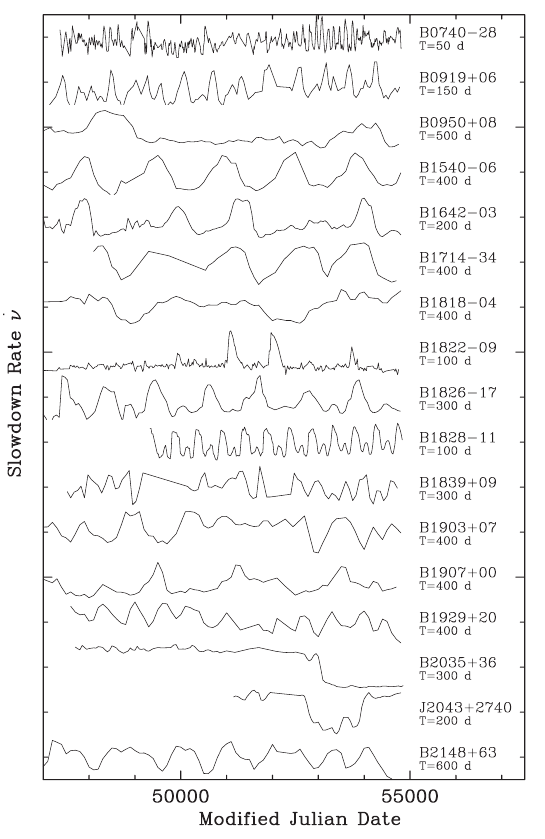
\includegraphics[width=.5\textwidth]{Lyne_2010_fig2}
    \caption{Figure taken from \citet{Lyne2010} showing the spin-down rate
             of 17 pulsars over a $\sim20$~year period.}
    \label{fig: lyne 2010 fig2}
\end{figure}

The method used to calculate the spin-down in Fig.~\ref{fig: lyne 2010 fig2}
required time averaging; the baseline used $T$ is given below the pulsar name
on the right-hand side of the plot, typically $T\sim100$~days. The authors of
\citet{Lyne2010} argue that, if the pulsar is in fact switching between
magnetospheric states then its spin-down rate will be periodically switching
between at least two values. In the event that the switching occurs over
timescale comparable the time averaging baseline, the resulting time averaged
spin-down will be smoothed out. Therefore, the smooth periodic variations in
Fig.~\ref{fig: lyne 2010 fig2} could be produced by the spin-down rate
switching between two (or more) well defined values.

If the switching was magnetospheric in origin, then \citet{Lyne2010} realised
that changes in the spin-down rate should correlate with changes in the
beam-shape.  They found that for 6 pulsars the pulse width did indeed correlate
with changes in the spin-down rate, although not always with the same
directionality.  However, like the spin-down rate these pulse shape variations
are also smooth and subject to the same averaging process.

To test if the mechanism causing these variations is smooth or instantaneous
(i.e. switching) the authors needed to look at an observed property not subject
to the time-averaging process.  This is possible by looking at individual
measurements of the pulse width which are taken during each short $\sim30$~mins
observation. In this way they are time averaged over a duration much shorter
than the modulation period and could, in principle, resolve individual
switching events. They were able to do this for two pulsars B1822-09 and
B1828-11 and argues that the individual beam-width measurements, by eye, can be
interpreted as taking one of two values with few observations seen in between.
They took this as evidence that the pulsars were indeed undergoing sudden,
instantaneous, and periodic switching between two states.

Since this initial study, evidence for switching in two others pulsars have
been reported by \citet{Perera2014} and \citet{Perera2016} with additions added
to the model in terms of the detail of the switching. However, so far the
magnetospheric switching hypothesis is missing an underlying physical model
which both causes the switching between states and provides the clock regulating
the period.

\citet{Lyne2010} argue that the fast state changes seem to rule out free
precession as the origin of oscillatory behaviour observed in timing residuals.
One of the pulsars which shows some evidence for two state switching is PSR
B1828-11; this pulsar was cited as evidence for free precession by
\citet{Akgun2006}. \citet{Lyne2010} argue that the fluctuations from this pulsar
should be reinterpreted as two-state switch due to the observed fast state
changes.

\citet{Jones2012} argues that such dismissal of precession is premature since
the modulation period of the switching has yet to be explained.  Instead, the
author raises the idea that precession and magnetospheric switching are not
mutually exclusive, but precession may in fact cause the switching. Pulsars are
most probably born in a randomly distributed magnetospheric state, at least
some may therefore exist under a delicate balance between two states.
Precession may be capable of periodically varying the statistical probability
of existing in one state or the other, sharp changes would be caused by an
`avalanche effect' as the particle energies reach a threshold.  This provides
the timescale for switching along with the ability for the switching to be
quasi-periodic since the precession only biases the probability.

A alternative idea proposed by \citet{Cordes2013} interpreted two state
switching as evidence for a system in a state of `stochastic resonance'.  This
occurs in systems in which, under certain conditions, a weak periodic forcing
function is amplified by stochastic noise. To explain this phenomenon in
appendix \ref{app: stochastic} we present a toy model of stochastic resonance
for a particle in a well. The switching could therefore be the result of any
periodic modulation, such as precession, coupled to random fluctuations. This
would quite naturally explain the stability of states, the timescales over
which the occur, and the fact that it is observed in only some pulsars.

In Chapter~\ref{sec: testing models} we present as quantitative
model comparison of magnetospheric switching with precession for PSR B1828-11.
In the following sections we will present the basics of the empirical switching
model and then develop an idea of how pulsar astronomers could test for switching.

\subsubsection{Simple empirical model}

In the supplementary material to \citet{Lyne2010}, the authors presented
results from a simple empirical switching model to demonstrate the resulting
phase residuals. In this section we will similarly develop a simple model and
show the effecting of switching on the time-averaged spin-down rate and phase
residuals.

Firstly we model a pulsar as spinning down in the usual way except that its
spin-down switched between two distinct values $\dot{\nu}_{A}$ and $\dot{\nu}_{B}$
staying in each for $t_A$ and $t_B$ respectively; we use
$A$ and $B$ to denote the two magnetospheric states. Then, we
define the ratio of time spent state in state $A$ and $B$ as $R =
t_{B}/t_{A}$.  This is a purely deterministic model and, having generated the
spin-down values, we can integrate twice to get the phase. From the phase, we can
use the method of \citet{Lyne2010} (described in Sec.~\ref{sec: switching})
to get the time-averaged spin-down rate $\langle\dot{\nu}\rangle$, or we can
fit a polynomial to the entire phase evolution and remove it to get a phase
residual.

In Fig.~\ref{fig: lyne example D=0} we show the underlying spin-down rate $\dot{\nu}$,
the time-averaged $\langle\dot{\nu}\rangle$, and phase residual (in cycles) for
some typical values. For the time-averaged spin-down rate we carefully chose
an averaging time similar to the switching period. For the final phase residual
we fit and remove a Taylor expansion up to $\ddot{\nu}$ and divide the residual
difference by the period in order to get the phase residual in cycles.
\begin{figure}[htb]
    \centering
    \includegraphics[]{{R_3.0_D_0}.pdf}
    \caption{A deterministic realisation of the Lyne switched spin-down model. The
             resulting structure in the time-averaged spin-down rate and the phase
             residuals are strictly periodic.}
    \label{fig: lyne example D=0}
\end{figure}

The phase residuals in figure \ref{fig: lyne example D=0} are strictly periodic
which is inconsistent with the observed variations in the majority of pulsars
\citep{Hobbs2010}.  To develop this, \citet{Lyne2010} added a probabilistic
'dither' $D$ in the waiting time between switches. Now we have periods
$t_{A}^{i}$ and $t_{B}^{i}$ which are Gaussian distributed with a mean of
$t_{A}$ and $t_{B}$ and a standard deviation $D t_{A}$ and $D t_{B}$. In
Fig.~\ref{fig: lyne example D=0.3} we repeat the results of Fig.~\ref{fig: lyne example D=0}
with $D=0.3$.
\begin{figure}[htb]
    \centering
    \includegraphics[]{{R_3.0_D_0.3}.pdf}
    \caption{A realisation of the Lyne model with a random element producing the
             observed quasi-period structure.}
    \label{fig: lyne example D=0.3}
\end{figure}

\subsubsection{Simple empirical model: four time periods}
The spin-down rates seen in Figs.~\ref{fig: lyne example D=0} and Fig.~\ref{fig:
lyne example D=0.3} result from having two spin-down rates and two durations
which the system spends in those states. These results can be contrasted with
the spin-down rates of B1828-11 seen in Fig.~\ref{fig: lyne 2010 fig2}.
With only the ingredients described by \citet{Lyne2010}, it is not possible
to consistently replicate the double peaked spin-down rate variations seen
for this pulsar. A similar problem was faced by \citet{Perera2014} for
PSR B0919+06 and the authors devised the following solution. Rather than introduce
a third spin-down state, they simply required that the system has four periods
instead of two as in the original \citet{Lyne2010} description. The system then
switches between the two states four times during a single cycle.

To illustrate this, in Fig.~\ref{fig: test lyne underlying} we show a single
cycle in which the four periods are $100$, $100$, $50$, and $100$ days.
\begin{figure}[htb]
    \centering
    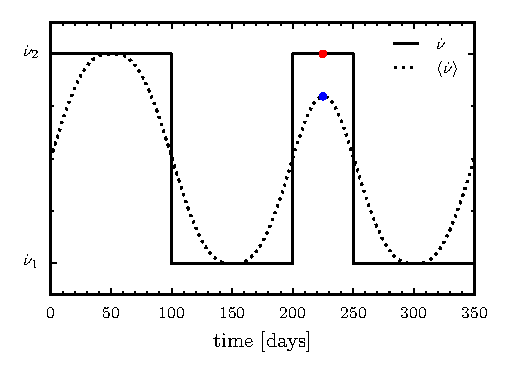
\includegraphics[]{TestLyneUnderlying}
    \caption{The spin-down rate $\dot{\nu}$ and its time-average $\langle\dot{\nu}\rangle$
    for a single cycle of the \citet{Perera2014} switching model in which the
    system switches between the two states four times during a single cycle.
    For the time-averaged spin-down rate, we have used a baseline for $100$~days,
    which is longer than the shortest period of 50~days; for this period we
    highlight the true spin-down rate by a red dot and the maximum time-average
    spin-down rate by a blue dot.}
    \label{fig: test lyne underlying}
\end{figure}

The \citet{Perera2014} switching model naturally produces the doubly peaked
time-averaged spin-down rate seen in B1828-11 when the time-averaging is longer
than one of the switching periods. To explain more fully, when the time
averaging baseline is longer than a single period, then the time-average over
that section of the data will always include some amount of the other spin-down
rate. This can be seen in Fig.~\ref{fig: test lyne underlying} for the third
period which has duration 50~days, while the time averaging baseline is
100~days. In Fig.~\ref{fig: perera example} we give the spin-down rate and
phase residual for this model to illustrate the variations in the residuals.
\begin{figure}[htb]
    \centering
    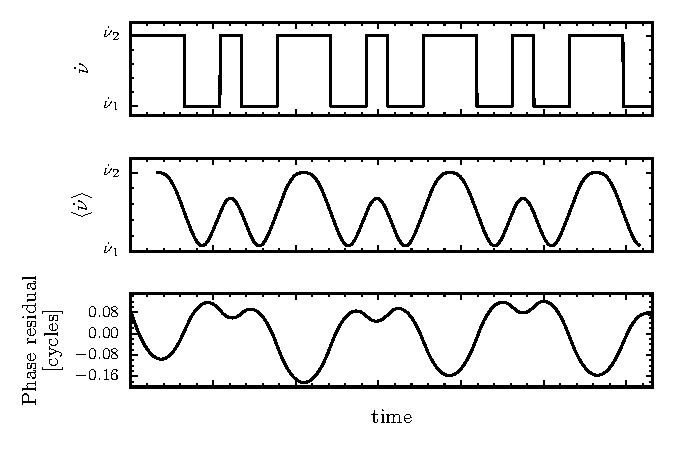
\includegraphics[]{Perera}
    \caption{Illustration of the \citet{Perera2014} extension to the
    \citet{Lyne2010} model in which the system switching between the two states
    four times per cycle, giving four independent switching periods.}
    \label{fig: perera example}
\end{figure}

In Sec.~\ref{sec: switching} we will consider this switching
model further in the context of B1828-11 and develop a complete model for the
spin-down rate and beam-width modulations.

\subsubsection{A simple test of the switching hypothesis}
PSR B1828-11, which has a distinct doubly peaked spin-down, is one of two pulsars
used in \citet{Lyne2010} as evidence of magnetospheric switching. We describe now
a simple method to test the switching hypothesis which so far, to our knowledge,
has not been tried.

If the double peaked spin-down rates of B1828-11, B0919+06, or any other pulsar
is due to model proposed by \citet{Perera2014}, then the maximum spin-down rate
of lower of the two peaks is a function of the time-averaging process and not
the pulsar itself.  Specifically, if the time-averaging was shorter than the
shortest period there would be no second, lower peak: both peaks would have a
value $\dot{\nu}$.  Therefore, if one had access to the original data used to
produce the time-averaged spin-down rate, one could repeat the time-averaging
process varying the time-averaging baseline which we denote by $T$. Then we
could imagine measuring the maximum spin-down rate of the two peaks in the
time-averaged spin-down rate and taking their ratio $R$. Then, if the Perera
switching model is to be believed $R$ should depend on $T$.

To demonstrate this, we can simulate the result numerically. That is, following
the method defined above, we generate the time-averaged spin-down rate and
calculate the spin-down rate of the second peak (the blue dot in Fig.~\ref{fig:
test lyne underlying}). Repeating this for a range of time-averaging baselines
we keep the underlying model fixed with the values used in Fig.~\ref{fig: test
lyne underlying}, then in Fig.~\ref{fig: test lyne} we plot the ratio $R$ of
the maximum spin-down rates of the two peaks.
\begin{figure}[htb]
    \centering
    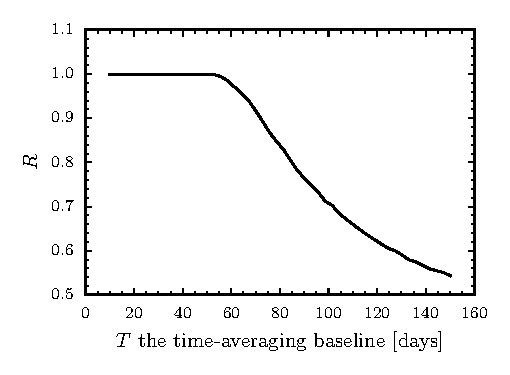
\includegraphics[]{TestLyne}
    \caption{Demonstrating of how to test the Perera switching hypothesis
             by varying the time-averaging baseline and measuring $R$ the ratio
             of the two peaks in the spin-down rate.}
    \label{fig: test lyne}
\end{figure}
This clearly shows that for $T\le50$~days the ratio $R=1$ because the two peaks
are of equal size, there is no reduction in the peak because the $T$ is shorter
than the shortest segment of length $50$~days. However, for $T>50$~days $R$
decays up to $T=150$~days, above this the time-averaging is of a similar length
to the total period of switching and so we can't resolve any of the features.
The important point here is that, if one observes a doubly-peaked spin-down
rate the Perera switching model can be tested by measuring the time-averaged
spin-down rate with two or more $T$ values: variations in the ratio of the
two peaks would provide clear evidence in favour of the model.


\subsection{Evidence from anomalous braking indices}
\label{sec: evidence from anomalous braking indices}

An alternative motivation to study timing noise comes from the measurement of
anomalous braking indices. The pulsar braking index is defined by $n$ in
equation \ref{eqn: power law spin-down}.  Rearranging this equation as in
\eqref{eqn: measured braking index} the braking index can be measured for
observed pulsars. Different types of braking exhibit different braking indices.
It is therefore a reasonable idea to measure the braking index and calculate
the type of braking. Pulsars spun down by an electromagnetic torque should
follow a braking index of $n=3$, while gravitational wave spin-down has $n=5$.

Measuring these indices for the known pulsar population we do not find a consensus
on the type of braking. Values from from unity up to $10^{6}$ and even negative
braking indices have been measured. These are known as \emph{anomalous}
braking indices.

Recent work by \citet{Biryukov2012} observed that
younger pulsars tend to have braking indices of the correct order of
magnitude. However, beyond~$\tau_{ch}\approx10^{5}$~years
the absolute value of the braking index rapidly grows,
reaching values as large as $10^{6}$ for the oldest pulsar. In addition an
almost equal number of pulsars have positive and negative values of the braking
index. The figure demonstrating this is plotted in
figure~\ref{fig: braking indices}.

\begin{figure}[ht]
\centering
	\includegraphics[width=0.5\textwidth,trim=0mm -10mm 0mm 0mm]
               {{Biryukov_2012_Figure_7}.png}
\caption{Pulsar population in the $n_{obs}-\tau_{ch}$ diagram image from
\citet{Biryukov2012}}
\label{fig: braking indices}
\end{figure}

\citet{Biryukov2012} proposed that the spin-down $\dot{\nu}(t)$ may contain the
secular spin down $\dot{\nu}_{\textrm{sec}}(t)$ and a cyclic component
$\dot{\nu}_{\textrm{sec}}(t)\epsilon(t)\nu(t)$ oscillating the spin-down about
a mean value. Taking a simple case where the cyclic term has the form $A
\cos\phi(t)$ where $A$ is the relative amplitude of the oscillations and
$\phi(t)$ is linear in $t$, the authors derive an equation for the observed braking
index

\begin{equation}
n_{obs}(t) =
\frac{n}{1+A\cos(\dot{\phi}t+\phi_0)}
+\frac{(n-1)(kt-c)}{(1+A\cos(\dot{\phi}t+\phi_{0}))^{2}}A\dot{\phi}\sin(\dot{\phi}t+\phi_{0}).
\label{eqn: nobs}
\end{equation}•

This observed braking index contains a constant positive term oscillating about
the true braking index and a term which grows linearly in time. The authors found
that for $\tau_{ch}<10^{5}$ yrs the linear term is negligible and so we observe
approximately the real braking index $n$. At later times the linear term
drives the observed braking index to larger values while a sinusoidal term produces
positive and negative values. In figure \ref{fig: nobs} we plot the trajectory
of a single pulsar following equation \eqref{eqn: nobs}. The authors claim each
of the pulsars in \ref{fig: braking indices} is following a similar trajectory.

\begin{figure}[ht]
\centering
	\includegraphics[width=0.5\textwidth]
               {{Analytic_Monotonic_and_Cyclic}.png}
\caption{A sketch of the observed braking index according to
equation \eqref{eqn: nobs}, the values here are intended for a qualitative
overview rather than analysis. }
\label{fig: nobs}
\end{figure}

This simplistic idea is able to explain some of the defining features of the
known pulsar population braking indices. This requires a mechanism to modulate
the spin-down over long timescales. By fitting their model to data, they
estimate the timescale to be of the order $10^{3}-10^{4}$~years. At least one
physical model, precession, could produce variations on the required timescale.
However, this is significantly longer than the precession timescales invoked to
explain the fluctuations in timing residuals which were $1-10$~years.
\begin{subappendices}
\subsection{Toy model of stochastic resonance: particle in a potential}
\label{app: stochastic}

Here we present a simple toy model of stochastic resonance. This is a
statistical phenomena occurring when a weak periodic forcing function is
amplified by noise (see \citet{Jung1991} for a full treatment).  For the
application to neutron stars, see \citet{Cordes2013}; here we simply aim to
describe the essential features of stochastic resonance (not its application to
NSs).

We will consider a particle at a position $x$ which is subject to some
potential and acted upon by a forcing function $F(t)$. In general though, $x$
could be any state variable, thus stochastic resonance could be produced
in many systems.

First consider the static case of a particle in a potential $U(x)$  given by:
\begin{equation}
    U(x) = \frac{x^{4}}{4}-\frac{x^{2}}{2}.
\end{equation}
This potential is characterised by two wells at $\pm1$, a maximum exists
between them at the origin. The particle in one of the wells sees a potential
barrier $\Delta U$ corresponding to the height of the maximum above its
position.

Assume the particle is acted upon by a random forcing function $F(t)$ which is
modelled as a Gaussian white noise with strength $D$. Depending on the
magnitude of $D$ with respect to the potential, the motion of the particle
admits two distinct cases:
\begin{enumerate}
\item $D \ll \Delta U \;\;$ in which case the particle remains inside whichever
    well it initially starts in and does not escape.
\item $D \gg \Delta U \;\;$ in this case the particle will not see the the
    individual wells only the larger one.
\end{enumerate}

The motion of the particle obeys the following equation of motion:
\begin{equation}
    \frac{dx}{dt} = -\frac{\partial V(x,t)}{\partial x} + F(t).
\end{equation}
The motion of the particle has two components, the deterministic effect of the
potential and random fluctuations.

We now modify the potential to be acted on by a weak periodic function; this
introduced a third possible type of behaviour. Writing the time dependant
potential as
\begin{equation}
    V(x,t) = \frac{x^{4}}{4}-\frac{x^{2}}{2} + \epsilon x \cos(\omega_{0} t).
\end{equation}
Inserting this potential into the equations of motion:
\begin{equation}
    \frac{dx}{dt} =  x - x^{3} + F(t) + \epsilon \cos(\omega_{0} t).
\label{eqn:stochastic eom}
\end{equation}
Solving this numerically we fix $\epsilon=0.001$,
$\omega_{0}=\frac{2\pi}{10}$ and choose three values of $D$ which illustrate
typical behaviours of the solution
\begin{figure}[ht]
\centering
   \includegraphics[width=0.4\textwidth,trim=0mm -10mm 0mm 0mm]
   {{Stochastic_resonance}.png}

\caption{Three solutions to equation \eqref{eqn:stochastic eom} changing the
    random forcing functions strength $D$. The first and last panels show the
    deterministic solutions for the particle position: either the forcing
    function is weak compared to the potential, the particle remains in well in
    which it begins; or the forcing function is much stronger than the
    potential and so the particle freely moves about the two wells. The middle
    panel illustrates the special case of stochastic resonance whereby the
periodic fluctuations of the potential allow quasi-periodic variations in the
particles position between the two wells.}

\label{fig:stochastic resonance}
\end{figure}
The first and last runs replicate the behaviour expected  for a static well,
either the particle is confined to the well it starts in, or the random noise
is too strong and the individual wells are not observed. The middle case
displays strong stochastic resonance: the solution
displays a switching between bi-stable states but does not strictly follow the
period of the forcing function. The
important point here is that the forcing function may be weak, but provided it
is periodic or at least quasi-periodic the signal is amplified by the random
noise such that it may be visible in data sets where it would typically be
considered lost.

\end{subappendices}
